\chapter{Библиотека TopicNet и её применение в конкретных задачах}

\subsection{механизм отбора моделей в TopicNet}
\subsection{multitask learning}
\subsection{рецепты}
“мы подготовили рецепт: мы берём комбинацию регуляризаторов и оно почти всегда работает хорошо из коробки”


\section{Introduction}

To facilitate the research on mining latent topics from texts and text-like collections, we present a novel software package called TopicNet\footnote{Source code can be downloaded from \url{github.com/machine-intelligence-laboratory/TopicNet} \par The documentation is available at \\ \url{machine-intelligence-laboratory.github.io/TopicNet} }. This software package contributes to the flexibility of topic model design and provides powerful out-of-the-box experience boosting the accessibility of topic modelling for the general audience.

\section{Related Work}

Existing topic modelling algorithms originate from latent semantic analysis approach~--- LSA \cite{deerwester1990indexing}, which is, in the essence, a singular value decomposition with the lowest possible rank for document$\times$term matrix. Later, a probabilistic approach took the main place in the topic modelling field.

A probabilistic topical model can be considered as a black box that receives a text document collection at the input and produces two families of distributions at the output: the term probabilities for each topics $\phi_{wt} = p(w \mid t)$ and the topic probabilities for each document $\theta_{td} = p(t \mid d)$. The term$\times$topic matrix $\Phi$ and topic$\times$document matrix $\Theta$ are model parameters to be found during the training.

The development of probabilistic topic modelling started with two fundamental models: probabilistic Latent Semantic Analysis~--- pLSA \cite{hofmann1999probabilistic} and Latent Dirichlet Allocation~--- LDA \cite{blei2003latent}. LDA adds Dirichlet prior to pLSA: the generative LDA model draws term-topic and topic-document distributions from prior Dirichlet distributions, each with its own concentration parameter. While writing a document, authors usually use only handful of topics per each text. This sparsity property is reflected in concentration parameter. Varying value of this parameter, one can obtain distributions where only a few topics have high probability to be in a document with other topic probabilities being small. Thus, the sparsity of Dirichlet distributions is the probabilistic tool that encodes this intuition. However, according to the article \cite{wallach2009rethinking}, LDA requires extensive hyperparameter optimization toward producing good results.

На протяжении последних десятилетий были разработаны сотни расширений моделей PLSA и LDA, 

Over the past years, hundreds of pLSA and LDA model extensions have emerged, each taking into account the various problem-specific data features and providing  desired solution properties. Starting with LDA model, Bayesian learning is the de facto standard in topic modelling. In this approach, one first describes the probabilistic generative model of data,

specifies prior distributions of the model parameters,

and then uses Bayesian inference to obtain the parameter posterior distributions. Bayesian inference method requires unique derivation and, consequently, unique implementation for each new model. 

% ### CHANGE ###

Аддитивная регуляризация тематических моделей (АРТМ, ARTM) \cite{voron14dan-eng,kochedykov2017fast} --- небайесов многокритериальный подход. 

Основанный на максимизации правдоподобия, сложенного с взвешенной суммы произвольных функций (регуляризаторов). Многие байесовы модели могут быть проинтерпретированны как модель PLSA, подвергнутая какой-либо регуляризации. За счёт аддиктивности подход АРТМ позволяет комбинировать множество регуляризаторов внутри одной тематической модели. Эта модулярная технология реализована внутри откртой библиотеки BigARTM \footnote{\url{bigartm.org}} 
\cite{voron15aist}. 

Given a generative model and data, inference must be executed for extracting probabilistic topic-depending distributions. There are many inference algorithms: expectation-maximization (EM) algorithm, Gibbs sampling, variational inference, gradient descent and message passing. In ARTM the regularized EM-algorithm is used to learn model parameters. The similarities between each of the algorithms were noted before in \cite{asuncion09smoothing}. 

Gensim \cite{rehurek_lrec} --- наиболее популярный фреймворк для тематического моделирования. В нём реализован ряд известных моделей (LSA, pLSA, LDA, Hierarchical Latent Dirichlet Allocation (HLDA) и их производные). Также эта библиотека предоставляет интерфейс измерения когерентности по верхним токенам темы, основанный на работе \cite{roder2015exploring}. Gensim написан на языке Python и оптимизирован для работы с большими коллекциями документов. 

Stanford Topic Modelling Toolbox~--- STMT \cite{stanfordtmt}, написанный на Scala, поддерживает обучение LDA, Labelled LDA и PLDA. Полезной особенностью Stanford TMT является интеграция с Excel.

MALLET \cite{mccallum2002mallet} --- классическая реализация тематического моделирования, написанная на Java и основанная на сэмплировании Гиббса. 
Инструментарий MALLET позволяет строить модели LDA, Pachinko Allocation \cite{li2006pachinko}, и HLDA. Часто используется для онлайн-сервисов \cite{pol2017towards}.

A Library of Short Text Topic Modelling (STTM) \cite{qiang2018sttm} ~--- написанный на Java фреймворк, предназначенный для работы с коллекциями коротких текстов. Данный пакет поддерживает множество специализированных моделей: Dirichlet Multinomial Mixture DMM \cite{yin2014dirichlet}, Word Network Topic Model WNTM \cite{zuo2016word}, Pseudo-Document-Based Topic Model PTM \cite{zuo2016topic} and Self-Aggregation-Based Topic Model SATM \cite{quan2015short}. Также поддерживаются некоторые модели, предназначенные для работы с длинными текстами: LDA и Latent Feature Model with LDA \cite{nguyen2015improving}.

Familia \cite{jiang2018familia} --- фреймворк, поддерживающий LDA и Supervised LDA: Topics Over Time TOT \cite{wang2006topics}, Bilingual Topic Model \cite{gao2011clickthrough}, Location-Aware Topic Model LATM \cite{wang2007mining}. Авторами было заявлено, что Familia даёт возможность ``проектировать свои собственные тематические модели'', используя смплирование Гиббса как механизм вывода. К сожалению, репозиторий на GitHub такую функцию не поддерживает: в открытом релизе отсутствует возможность построить пользовательскую тематическую модель и даже возможность обучить предоставленные модели на пользовательской коллекции \cite{familia_github}.

Known to us, two software packages implement a number of metrics and operate on a similar idea:  they allow the user to explore the values of several quality metrics among the range of different $T$ and select a point that appears most advantageous.

The \texttt{ldatuning} package\footnote{https://github.com/nikita-moor/ldatuning} for R \cite{ldatuning} has 4 methods supported:  D-Spectral \cite{arun2010finding}, D-avg-COS \cite{cao2009density}, D-avg-JS \cite{deveaud2014accurate}, and holdPerp \cite{griffiths2004finding}. It depends on the \texttt{topicmodels} package, which supports LDA and CTM models. The recent work of \cite{hou2018benchmarking} examines the performance of these methods on several generated datasets with a known value of $T$.

The TOM library\footnote{https://github.com/AdrienGuille/TOM} for Python \cite{guille2016tom} implements 3 methods for estimation of $T$: D-Spectral \cite{arun2010finding}, toptokens-ssample-stab \cite{greene14howmany}, and cophenet \cite{Brunet4164}.  It supports Latent Dirichlet Allocation models and models based on Non-negative Matrix Fac\-tor\-iza\-tion.

Как было замечено выше, высокий порог входа в область тематического моделирования для потенциальных пользователей по-прежнему остаётся важной проблемой, которую необходимо решить. Ситуация ещё более осложняется, если пользователю необходимы не классические модели, доступные в самых популярных фреймворках (Gensim, MALLET), а более продвинутые их модификации.

Другой аспект этой проблемы --- построение новых тематических моделей с нуля. Самостоятельно реализовать классические тематические модели сравнительно несложно и доступно любому пользователю с навыками програмирования. Однако, эффективное построение комплексных многокритериальных моделей требует больших затрат времени и усилий (при этом трудно гарантировать вычислительную эффективность и отсутствие программных ошибок) \cite{jiang2018familia}.

Цель библиотеки TopicNet --- сделать имеющийся инструментарий тематического моделирования более доступным для широкой публики и облегчить конструирование новых тематических моделей.

% Due to ARTM formalism, TopicNet offers natural language processing community access to Python-based multimodal topic modelling that supports large documents and huge corpora. 

\section{Технология в основе}

Библиотека TopicNet --- это высокоуровневая надстройка над библиотекой BigARTM. Мы более детально рассмотрим плюсы библиотеки \mbox{BigARTM} и её минусы, которые мы надеемся компенсировать посредством библиотеки TopicNet.

\subsection{Достоинства BigARTM}

% ### CHANGE ###

BigARTM --- быстрая и гибкая библиотека для тематического моделирования \cite{frei2016parallel}, основанная на формализме Additive Regularization of Topic Models (ARTM) \cite{voron14dan-eng}. Идея подхода состоит в том, чтобы перейти от оптимизации правдоподобия к оптимизации регуляризованного правдоподобия (использя модифицированный EM-алгоритм). 
Регуляризация выполняет две цели. Во-первых, она обеспечиывает устойчивость за счёт накладывания дополительных ограничений на решение. Во-вторых, каждый дополнительный регуляризатор позволяет указать на желательность каких-то дополительных свойств модели: например, разреженность распределений, различность тем, когерентность верхних токенов. 

Также регуляризация может учесть какую-то дополнительную информацию. Чаще всего встречающийся на практике случай --- использование метаданных документа (e.g. authors, timestamps, tags, and n-grams). Воспользоваться этой информацией в рамках подхода АРТМ оказывается существенно проще, чем в байесовых подходах: правдоподобие каждой дополнительной модальности можно рассматривать как регуляризатор, аддитивно применённый к тематической модели над множеством слов \cite{voron15nonbayesian}.

Список работ, использующих гибкость ARTM и BigARTM включает в себя: улучшение качества разведочного поиска \cite{yanina17technews}, 
построение интерпретируемых тематических представлений слов посредством модели сети слов \cite{potapenko17interpretable}, 
иерархическое тематическое моделирование \cite{chirkova16additive}, 
улучшение представлений документов для задач текстовой регрессии \cite{sokolov15topic}, 
нахождение редких этнорелевантных тем в социальных сетях \cite{apishev16additive,apishev16mining}, 
использование лингвистических признаков \cite{popov_hier}, отбор тем при помощи разреживащей энтропийной регуляризации \cite{voron15slds}, улучшение тем при помощи сегментации текста \cite{skachkov}, 
прямая оптимизация когерентности верхних токенов \cite{4keys}, 
отход от гипотезы мешка слов за счёт использования определённой метрики качества \cite{intracoh}. 
Обзор \cite{kochedykov2017fast} показывает, как байесовы тематические модели (в том числе multimodal, multilingual, temporal, hierarchical, graph-based, and short-text topic models) могут быть переформулированы в терминах подхода АРТМ.

Разработка как теории АРТМ так и библиотеки \mbox{BigARTM} продолжается и по сей день. Многие существующие регулризаторы были вкладом со стороны сообщества.

Насколько нам известно, по гибкости BigARTM превосходит все остальные фреймворки для тематического моделирования. Из перечисленных выше аналогов лишь Familia заявляет о сравнимом функционале; при этом в открытом релизе Familia такой функционал отсутствует \cite{familia_github}.

\subsection{Недостатки BigARTM}

Оптимизации, направленные на вычислительную эффективность, делают BigARTM мощным инструментом, который, однако, имеет ограниченную область применимости. Если пользователь уже имеет точное описание требуемой регуляризованной модели, то библиотека BigARTM способна очень быстро выучить её параметры $\Phi$, $\Theta$. К сожалению, наличие таких готовых спецификаций --- редкость.

Число тем -- гиперпараметр, самый распространённый среди различных тематических моделей. Все средства для тематического моделирования предоставляют пользователю возможность указать этот гиперпараметр; большинство из них не дают никаких рекомендаций по выбору хорошего значения. Много работ посвящено этому вопросу.

В подходе АРТМ ситуация ещё далее ухудшается; в самом деле, теперь пользователь может скомбинировать произвольное число регуляризаторов, каждый из которых имеет индивидуальный коэффициент регуляризации (а также возможно какие-то другие структурные параметры). Всё это дело никак не регламентируется.

Второй фактор, увеличивающий порог входа --- местами неудобность интерфейса библиотеки. Это естественный итог того, что новый экспериментальный функционал разрабатывался и встраивался в библиотеку до того, как сообществом были выработаны "лучшие практики" по его применению (а также желания сохранить обратную совместимость). 

% Так получается парадоксальный результат: Therefore, as applications of \mbox{BigARTM} were becoming more diverse and the algorithms were gradually refined, the high-level interface of \mbox{BigARTM} was getting less well-suited for ``best practices''.

Ещё одна проблема библиотеки BigARTM --- сложность её расширения. С технической точки зрения, библиотека BigARTM состоит из высокопроизводительного ядра, написанного на C++ и ряда классов-обёрток на языке Python. Реализованные на C++ низкоуровневые функции тщательно оптимизированы, многопоточны --- всё это даёт BigARTM превосходство в скорости. С другой стороны, это затрудняет понимание и изменение этого фундаментального низкоуровневого кода. Высокоуровневый интерфейс не всегда предоставляет достаточную гибкость (например, для испытаний пользовательских регуляризаторов)

\section{Мотивация и видение}

Главная мотивация TopicNet --- создать инструмент, удобный как для новичков, так и для продвинутых пользователей. Эти две группы пользователей не обязаны использовать библиотеку одним и тем же образом; важнее всего обеспечить возможность взаимодействия групп друг с другом. Нами был сформулирован ряд требований, необходимых для достижения этой цели:

\begin{itemize}
\item{Модулярность: библиотека должна быть организована как совокупность независимых блоков, каждый из которых можно использовать в отрыве от остальных. Это требование обусловлено двумя причинами. Во-первых, это упрощает переход на новую технологию: продвинутые пользователи могут получить какую-то пользу от использования TopicNet, не внося радикальных правок в существующие проекты. Во-вторых, это необходимо для создания активного сообщества пользователей и разработчиков TopicNet: программмные проекты с понятной структурой более привлекательны для участников-контрибьюторов.}

\item{Инструменты визуализации: библиотека должна предоставлять пользователю набор мощных инструментов для визуализации. 
Такие инструменты играют важную роль при отладке и анализе ошибок, а также могут быть полезны для итоговых прикладных задач (например, показ похожих документов может быть нужен для отладки или непосредственно быть костяком системы разведочного поиска). 
Согласно вышеописанному требованию модулярности, этот инструментарий должен быть самодостаточным и иметь возможность развиваться в отрыве от остальной кодовой базы TopicNet.}

\item{Краткость: библиотека должна скрыть от пользователя низкоуровневые детали, давая возможность сосредоточиться на более существенных проблемах. Важно улучшить творческий процесс построения модели для решения конкретной задачи. 

Второе соображение в пользу этого решения основывается на принципе ``Соглашения по конфигурации'' (``convention over configuration''). Уменьшая количество вещей, требующих явной настройки, и предоставляя разумные значения по умолчанию, можно ``привить'' пользователю принятые в сообществе лучшие практики (такие, как сохранение построенных моделей или хранение данных для разных коллекций в разных директориях).

Третье преимущество заключается в читаемости и портируемости. Работая с более сжатым и регулярным кодом, пользователь может видеть бОльший объём кода в рамках экрана, что улучшает понимание эксперимента. В результате становится легче обсуждать, изучать и отлаживать эксперименты, а также делиться ими.}

\item{Работа ``из коробки'': в состав библиотеки должны входить схемы тренировки моделей, готовые к использованию и дающие приемлемый результат. Эти схемы должны подытоживать найденные сообществом стратегии решения определённых задач. Это обеспечивает пользователю-новичку положительный опыт первого взаимодействия с библиотекой и предоставляет продвинутому пользователю средство компактной записи для своих наработок.}

\end{itemize}

\section{Архитектура}

Библиотека TopicNet состоит из двух больших модулей: \texttt{viewers} и \texttt{cooking machine}. 

Модуль \texttt{Viewers} содержит различные инструменты визуализации. Дизайн придерживается философии Unix: каждый вьювер имеет ограниченную область ответственности и способен возвращать результат операции в JSON-подобном виде. 
Это даёт возможность комбинировать содержащиесся в модуле вьюверы, не теряя при этом удобные для конечого пользователя методы, возвращающие \texttt{pandas.DataFrame}, строку сформированного HTML, или отображающие результат сразу в ячейке вывода Jupyter Notebook. Примеры вывода TopTokensViewer и DocumentClusterViewer приведены на Рис. \ref{top_tokens} и \ref{documents_clusters} соответственно.

\begin{figure*}[h]
    \centering
    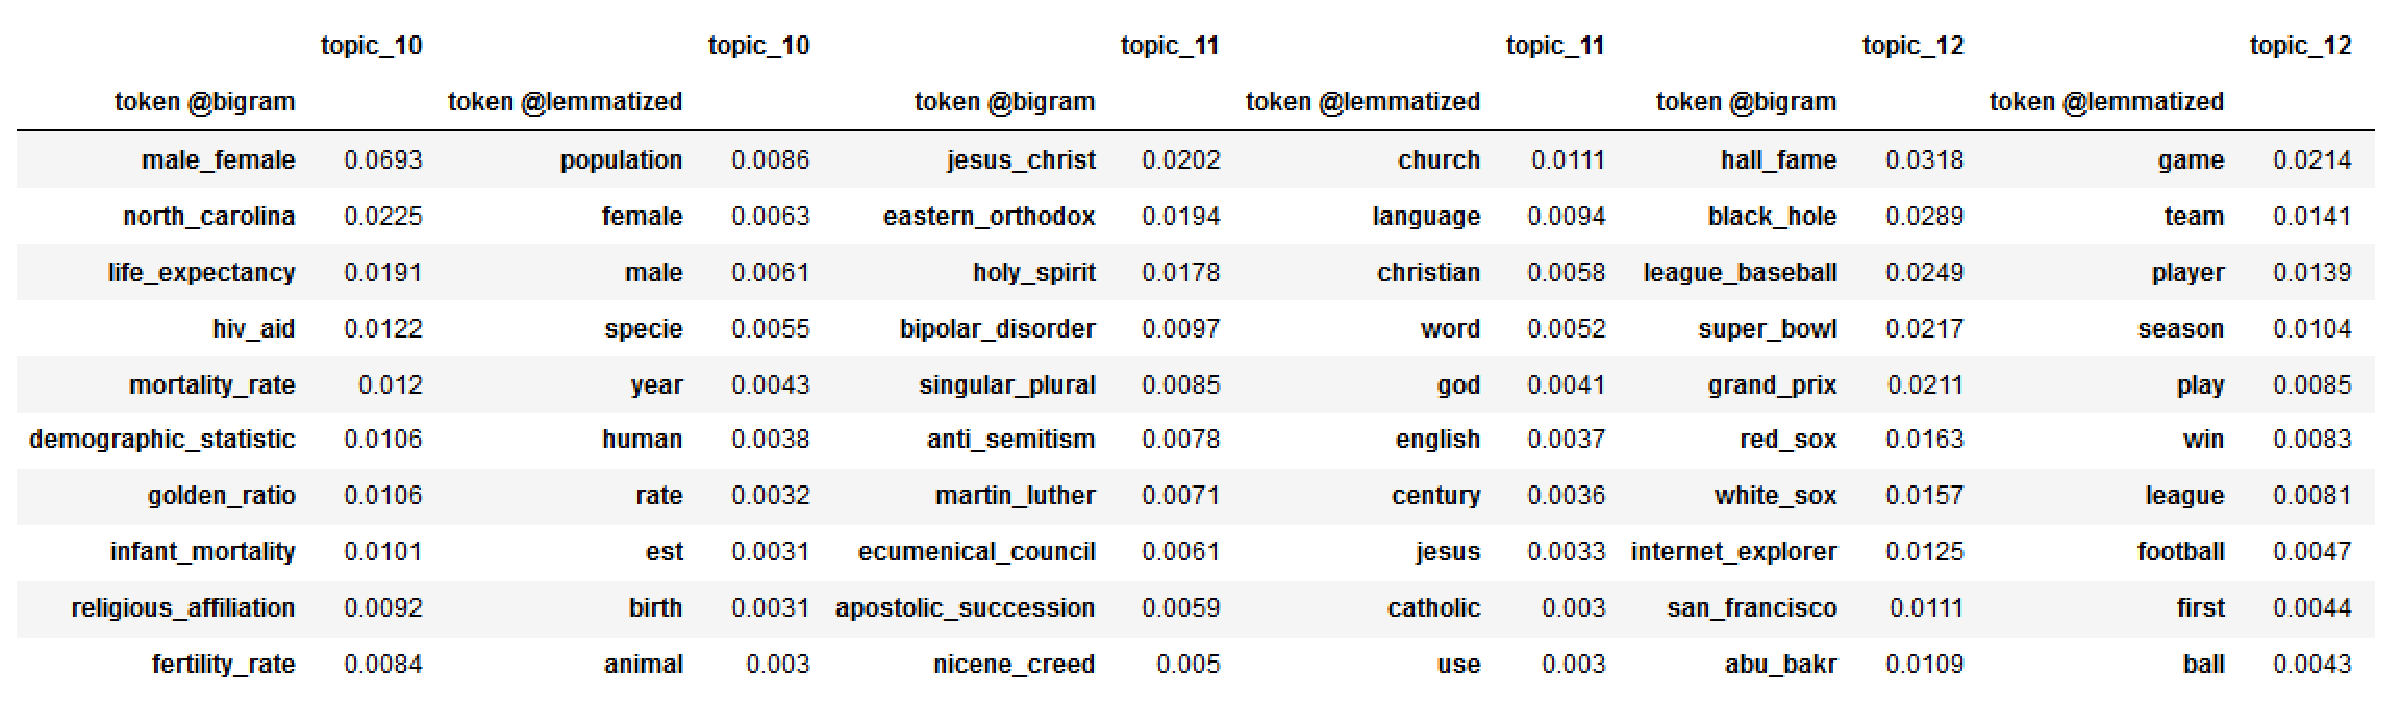
\includegraphics[width=0.98\textwidth]{sorted_3_topics.eps}
    \caption{Output of the TopTokensViewer. Token score in the topic is calculated for every token, score function can be specified at the stage of a viewer initialization.}
\label{top_tokens}
\end{figure*}

\begin{figure}[h]
    \centering
    \includegraphics[width=0.5\textwidth]{cluster_plot.eps}
    \caption{Visualisation of reduced document embeddings colored according to their topic made by DocumentClusterViewer.}
\label{documents_clusters}
\end{figure}

% Examples? common tasks such as TopTokenViewer and TopDocumentViewer and more sophisticated ones like SimilarDocumentViewer, TopicSpectrumViewer

% The library supports a variety of visualisation tools both conventional, such as top tokens and top documents viewers, and experimental ones.

Модуль \texttt{Cooking Machine} содержит различные инструменты для моделирования, 
embodied in the semi-hierarchical structure of the main modelling classes. 
These classes are responsible for building and training model of the given structure, for selecting models according to various constraints and for saving, loading and logging through the modelling process.

Following our ``convention over configuration'' principle, we enforce some assumptions on which kind of experiments TopicNet supports. 
Мы исходим из допущения о том, что процесс построения тематической модели представим в виде дерева. Каждый узел дерева содержит в себе тематическую модель, а ориентированные рёбра хранят информацмю об отношениях ``предок-потомок'' вида ``модель $Y$ была получена из модели $X$ при помощи преобразования $T_{XY}$''. Не все деревья эксперимента являются допустимыми. Мы накладываем ограничения на допустимые преобразования: мы требуем, чтобы все рёбра одного уровня описывали преобразования из одного и того же семейства, различающиеся лишь набором параметров. 

\newpage 
Возможые примеры таких преобразований:

\begin{itemize}
    \item Применить к модели регуляризатор с произвольными параметрами (или изменить параметры существующего регуляризатора)
    \item Запустить процесс обучения модели на какое-то количество итераций
    \item Добавить в текущую модель несколько тем, обнаруженных внутри другой коллекции
\end{itemize}

\begin{figure}[t]
    \centering
    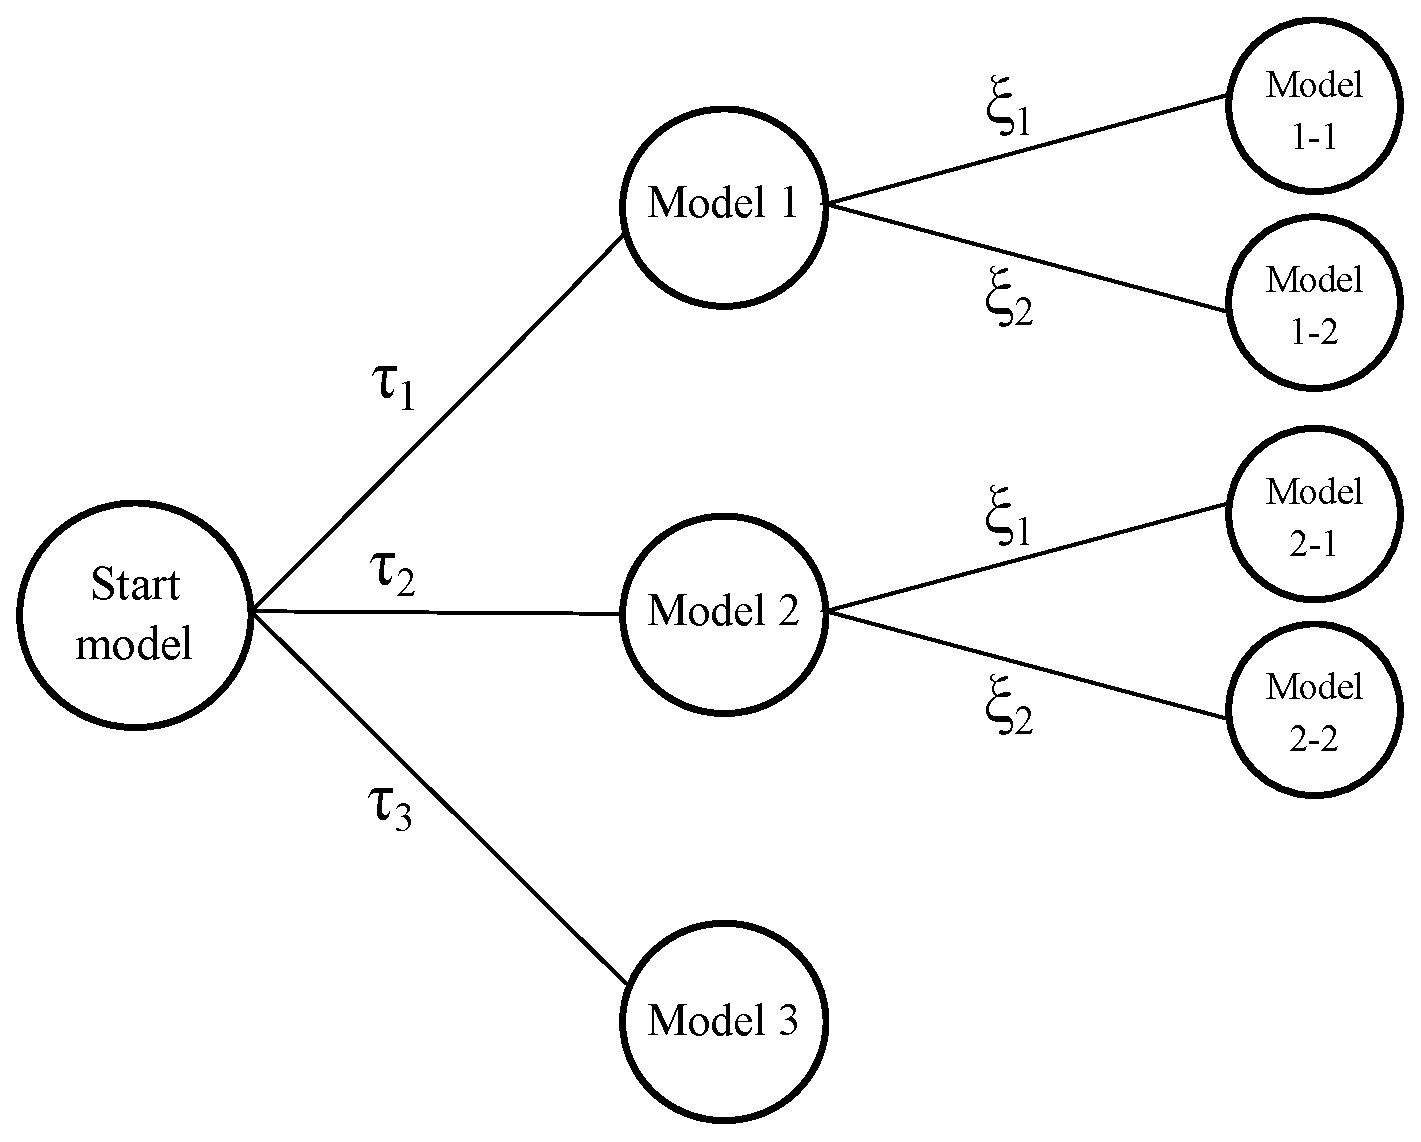
\includegraphics[width=0.4\textwidth]{training_scheme_example.eps}
    \caption{
        Example of the two-stage experiment scheme.
        At the first stage, regularizer with parameter $\tau$ taking values in some range $\{\tau_1, \tau_2, \tau_3\}$ is applied.
        Best models after the first stage are \emph{Model 1} and \emph{Model 2}~---~so \emph{Model 3} is not taking part in the training process anymore.
        The second stage is connected with another regularizer with parameter $\xi$ taking values in range $\{\xi_1, \xi_2\}$.
        As a result of this stage, two descendant models of \emph{Model 1} and two descendant models of \emph{Model 2} are obtained.
    }
\label{Training-scheme}
\end{figure}

\begin{figure*}[!ht]
\footnotesize
\texttt{TopicKernel@word.average\_contrast > 0.95 * MAXIMUM(TopicKernel@word.average\_contrast) \\
\hphantom{\ \ } and PerplexityScore@all < 1.1 * MINIMUM(PerplexityScore@all) \\
\hphantom{\ \ } and SparsityPhiScore@word -> max\\
\hphantom{\ \ } COLLECT 3}
\caption{This expression returns three models which are in the top 5\% according to contrast, has acceptable perplexity and as sparse as possible. \texttt{SparsityPhiScore} stands for the fraction of zeros in $\phi_{wt} = p(w \mid t)$ distribution.}
\label{DSL-example}
\end{figure*}


Класс \texttt{Experiment} отвечает за хранение, логгирование и актуализацию этой структуры. 

Все преобразования связаны с экземпляром класса \texttt{Cube}. Каждый \texttt{Cube} играет роль чертежа, задающего все преобразования на текущем уровне эксперимента. Таким образом, процесс обучения можно представить как цепочку кубов, последовательно соединённых друг с другом.

Куб выполняет две важные фукции. Первая --- это \textit{спецификация}: во время инициализации куб преобразует заданные пользователем параметры в многомерное пространство поиска. Вторая функция --- \textit{применение}: получив точку в пространстве поиска и тематическую модель, куб изменяет какое-то количество параметров и/или гиперпараметров модели. Таким образом, он играет роль инкубатора для моделей, что отражено в названии класса. На Рис.  \ref{Training-scheme} приведена схема обучения, состоящая из двух кубов, применённых к одной модели.

Классы \texttt{Experiment} и \texttt{Cube} позволяют сделать логгирование и сложные стратегии обучения более сжатыми и доступными. Модуль \texttt{config\_parser} делает ещё один шаг в сторону облегчения конфигурируемости: стратегию обучения можно задать при помощи текстового конфигурационного файла в формате YAML.

Другая область, описываемая пользователями как громоздкая и непрозрачная --- отбор моделей. В реальных экспериментах не у каждой модели есть потомки; большинство моделей отбрасываются в соответствии с каким-то критерием. Самый естественный, но в то же время самый трудозатратный способ --- это ручное изучение список верхних токенов и верхних документов, на основании которого пользователь принимает решение, какие из моделей являются ``удовлетворительными''. Другой подход заключается в сравнении численных показателей; обычно используется перплексия и когерентность. Библиотека \mbox{BigARTM} добавляет к их числу ещё какое-то число дополнительных метрик: например, разреженность, чистота и контраст \cite{voron15mlj}.

Для того чтобы облегчить груз ручной инспекции, мы реализовали простой domain-specific язык для отбора моделей (пример приведён на Рис \ref{DSL-example}). Результатом этого становится более простой и прозрачный процесс отбора моделей, способый учитывать множество критериев одновременно.

\section{Сравнение с конкурентами}

Сравнение TopicNet с другими фреймворками затрагивает несколько важных аспектов. Во-первых, было нужно убедиться в том, что обучение одной модели не занимает слишком много времени и не требует слишком много ресурсов. Во-вторых, нужно оценить интерпретируемость и различность тем у каждой модели.

Эксперименты проводились на коллекции 20 newsgroups. По набору 10 верхних токенов каждой темы измерялись две характеристики: 

* Umass-когерентность, показывающая согласованность слов между собой. Измерение производилось при помощи сервиса Palmetto \footnote{\url{palmetto.aksw.org/palmetto-webapp} } \cite{roder2015exploring}. В предыдущих работах было показано, что когерентность коррелирует с интерпретируемостью тем \cite{mimno2011}.
* Коэффициент подобия Жаккара, показывающий различность полученных тем. Коэффициент подобия, равный нулю, означает что в верхних словах тем нет общих слов (то есть множества их верхних 10 токенов не пересекаются), а равенство его единицы означает, что все темы являются полными дубликатами.

\subsection{Использование ресурсов}

Использование вычислительных ресурсов является фактором, который может затруднить широкое распространение фреймворка (например, студенты могут не иметь доступа к большим вычислительным мощностям; промышленное  использование также требует высокой скорости работы и низкой нагрузки на машину). Это сравнение будет проводиться на более крупном датасете NIPS \cite{mccallum1996bow}. 
 
\begin{table}[h]
\begin{tabular}{|l|l|l|}
\hline
                      & \multicolumn{1}{c|}{RAM, MB} & \multicolumn{1}{c|}{Training time, s} \\ \hline
TopicNet              & 991                         & 222.6 (15)                             \\ \hline
TopicNet multiprocess & 1084                        & 51.4 (15)                              \\ \hline
Gensim LDA            & 3559                        & 282.3 (3)                              \\ \hline
STTM DMM              & 3202                        & 52997 (1)                              \\ \hline
STTM PTM              & 1604                        & 84677 (1)                              \\ \hline
STTM WNTM             & 18663                       & 157819 (1)                             \\ \hline
\end{tabular}
\caption{In the first column we consider all the memory taken by the process during the training. The second column represents time needed to complete the training and number of models trained during the session.}
\label{performance-benchmark}
\end{table}

Как видно из таблицы \ref{performance-benchmark}, даже однопоточная версия превосходит конкурентов в скорости; испоьзование нескольких процессоров незначительно увеличивает расход оперативной памяти, но намного ускоряет процесс обучения. Таким образом, TopicNet не добавляет слишком много дополнительных расходов по сравнению с чистой библиотекой BigARTM.

\subsection{Model Quality} 

Следуя изложенным выше целям, мы предоставляем рецепт \texttt{ARTM baseline}, предназначенный для первого знакомства с библиотекой. Чтобы проверить качество этого рецепта, мы сравним модель, полученную посредством рецепта \texttt{ARTM baseline} с моделями ``по умолчанию'' из других фреймворков. Модели LDA и STTM были построены на 20 темах, модель TopicNet состояла из 19 предметных тем и одной фоновой. Никакой дополнительной настройки гиперпараметров не производилось (код тренировки модели приведён на \ref{topicnet_baseline}). 

% for TopicNet model we set 19 topics and one ``background'' topic, which has a special set of regularizers to collect polythematic documents. 


\begin{figure}[!ht]
    \centering
    \includegraphics[width=0.4\textwidth]{topicnet_baseline.eps}
    \caption{Example of the TopicNet baseline experiment.}
\label{topicnet_baseline}
\end{figure}

\begin{table}[h]
\begin{tabular}{|l|l|l|}
\hline
           & \multicolumn{1}{c|}{\begin{tabular}[c]{@{}c@{}}Jaccard measure\\ of topic dissimilarity\end{tabular}} & \multicolumn{1}{c|}{\begin{tabular}[c]{@{}c@{}}Average topic\\ coherence\end{tabular}} \\ \hline
TopicNet   & \textbf{0.00169}                                                                                               & -2.551                                                                                 \\ \hline
Gensim LDA & 0.01374                                                                                               & -2.747                                                                                 \\ \hline
STTM DMM   & 0.37541                                                                                               & -2.726                                                                                 \\ \hline
STTM PTM   & 0.02485                                                                                               & \textbf{-2.510}                                                                                 \\ \hline
STTM WNTM  & 0.01997                                                                                               & -3.572                                                                                 \\ \hline

\end{tabular}
\caption{Topic quality comparison}
\label{topic-comparisson}
\end{table}

Как мы видим из таблицы \ref{topic-comparisson}, построенная TopicNet модель  оказывается на втором месте по интерпретируемости (рис. \ref{topics_distribution} показывает дополнительную информацию о когерентности) и на первом месте по критерию различности тем. Это объясняется регуляризатором декорреляции, используемом в рецепте \texttt{ARTM baseline}. Комбинация этого регуляризатора, используемого скора и механизма, следящего за повышением перплексии, позволила найти модель, удовлетворяющую несколько требований одновременно.

\begin{figure}[!ht]
    \centering
    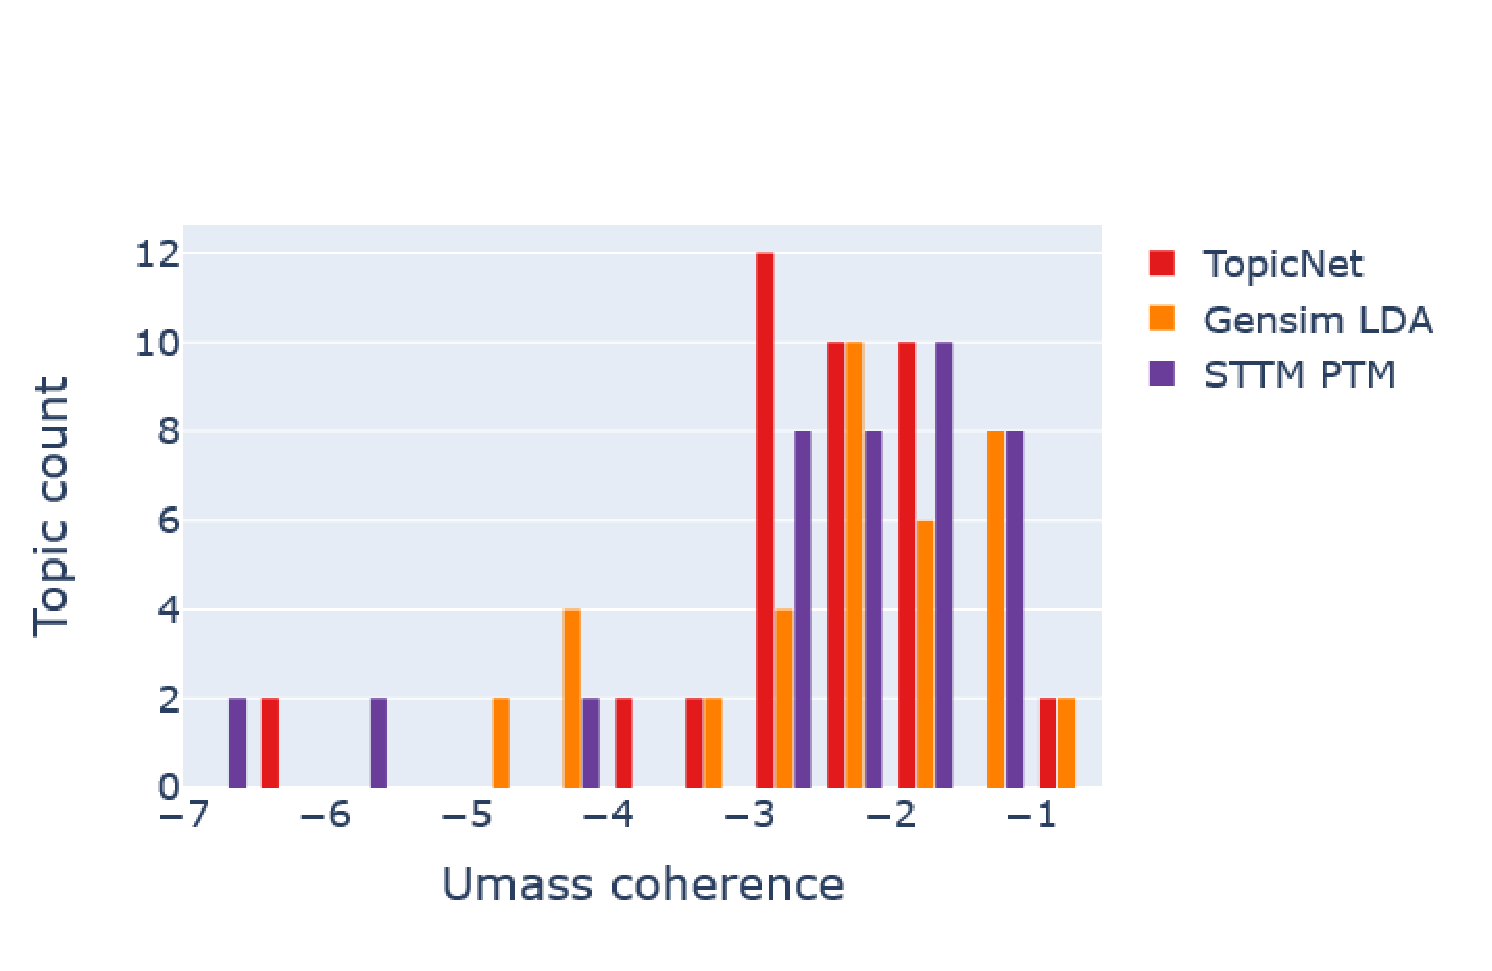
\includegraphics[width=0.45\textwidth]{Topics.eps}
    \caption{Распределение когерентности тем.}
\label{topics_distribution}
\end{figure}

%СРАВНИТЬ: 

%\begin{enumerate}
%    \item качество (используя наши вьюверы; нужно будет написать обёртку). Нужен хабр и техкранч от Насти.
%    \item Можно сравнить интерпретируемость? Или хотя бы когерентность.
%    \item hold out perplexity?
%    \item sparsity? Hence, disk space usage for final model.
%    \item RAM / CPU usage
%    \item Time
% \end{enumerate} 


\section{Заключение}
В этой главе был описан гибкий, конфигурируемый и быстрый фреймворк для подбора параметров и построения тематических моделей; показаны его преимущества по сравнению с другими фреймворками. TopicNet предоставляет широкий функционал: построение моделей с нуля, создние пользовательских скоров и регуляризаторов, возможность настройки параметров ранее построенных моделей.

Библиотека предоставляет готовые рецепты, отражающие лучшие практики построения АРТМ моделей под конкретную цель. Как было показано ранее, аддитивно регуляризованная модель способна превзойти модели конкурентов в терминах согласованных и не-повторяющихся тем. TopicNet помогает улучшить регулризованные модели дальше за счёт возможности введения пользовательских регуляризаторов и настройки гиперпараметров для мультикритериальных задач. 

При помощи комбинации BigARTM и TopicNet неспециализированный пользователь может реализовать новую тематическую модель, не встречавшуюсся в литературе раньше (другие фреймворки не позволяют этого добиться).

\todo{кажется, эти два абзаца надо переделать в полноценную секцию}

Помимо инструментов для гибкого и быстрого тематического моделирования, библиотека предоставляет средства контроля качества построенных моделей. TopicNet позволяет оценивать модели посредством различных встроенных метрик (скоров) и даёт возможность задать произвольные пользовательские метрики. Скоры могут вычисляться каждую итерацию тренировки, только на последней итерации, или с каким-то периодом. 

Также в состав библиотеки входит набор инструментов визуализации. К их числу относятся традиционные (top tokens and top documents viewers) и экспериментальные (спектр).

Библиотека TopicNet --- программный проект с открытым исходным кодом, имеющий потенциал для дальнейшего расширения. Модули \texttt{viewers} и \texttt{cooking machine} были спроектированы с учётом возможных улучшений со стороны сообщества в будущем.

Эти особенности дают основания верить в то, что эта библиотека будет одинаково полезна для software engineers и исследователей в области digital humanities.

